\documentclass[11pt,a4paper]{article}

\usepackage[T1]{fontenc}
\usepackage{lmodern}
\usepackage{microtype}
\usepackage[margin=2.5cm]{geometry}
\usepackage{graphicx}
\usepackage{float}
\usepackage{booktabs}
\usepackage{tabularx}
\usepackage{longtable}
\usepackage{amsmath,amssymb}
\usepackage{siunitx}
\usepackage{hyperref}
\usepackage{caption}
\usepackage{enumitem}

\hypersetup{hidelinks}
\captionsetup{font=small,labelfont=bf}
\graphicspath{{figures/}}

\title{Predicting High Income from Census Attributes}
\author{Adult Income ML Study}
\date{\today}

\begin{document}
\maketitle
\tableofcontents
\newpage

\textbf{A supervised machine-learning analysis of the UCI Adult / Census Income dataset}

\begin{quotation}
\textbf{Viewing figures:} Image paths are relative to this file (\texttt{./figures/...}). Open the preview from \texttt{reports/report.md} (not the repo root). If figures are missing, run \texttt{python scripts/03\_run\_eda.py} and later pipeline scripts, or \texttt{make eda} through \texttt{make report}.
\end{quotation}


\section{Introduction}

Income classification from census and survey variables is a longstanding benchmark in applied machine learning. The UCI Adult (Census Income) dataset records demographic, education, employment, and financial attributes for tens of thousands of individuals, with a binary label indicating whether annual income exceeds \$50,000. Predicting this label is useful as a methodological test bed for tabular classification, class imbalance, model comparison, and fairness auditing—not as a tool for individual-level decisions without further validation.

This report presents an end-to-end study: reproducible data preparation, exploratory analysis, comparison of classical and neural models, held-out evaluation, interpretability analysis, subgroup fairness diagnostics, calibration assessment, and an extension that removes sensitive attributes. Evidence is organised around a fixed traceability matrix linking each claim to tables, figures, or pipeline artifacts (see Appendix).


\section{Research Focus}

\subsection{Main research question}

\textbf{To what extent can income above \$50K/year be predicted from demographic, education, employment, and financial attributes in the Adult / Census Income dataset, and how do model family, preprocessing choices, calibration, interpretability, and subgroup fairness diagnostics affect the strength and reliability of that prediction?}

\subsection{Supporting objectives}

\begin{enumerate}
  \item Build a leakage-aware, reproducible binary classification dataset (DATA-001, DATA-002).
  \item Compare classical models and neural MLP variants under the same split and metric protocol (MODEL-001–005).
  \item Evaluate whether stronger predictive performance trades off against interpretability or subgroup disparity (INT-\textit{, FAIR-}).
  \item Produce an evidence-first report with traceable figures and tables (RPT-001).
\end{enumerate}

\subsection{Model selection criterion}

Models are compared using \textbf{mean 5-fold cross-validated macro F1 on the training split only}. The held-out test set is used once for final evaluation of the selected model (EVAL-001). Hyperparameters are tuned via randomized search on the training data; the test set is never used for selection or tuning.


\section{Dataset and Task Validity}

\subsection{Source and task definition}

Data were fetched reproducibly from the UCI ML Repository (id=2) via \texttt{ucimlrepo} (DATA-001). The prediction task is binary classification: \textbf{income ≤ \$50K (label 0)} vs \textbf{income > \$50K (label 1)}.

\subsection{Cleaning summary}

After cleaning (DATA-002), the analysis dataset contains \textbf{48,813} rows and \textbf{15} columns. Key steps are summarised in Table 3:

\begin{table}[H]
  \centering
  \small
  \begin{tabular}{ll}
    \toprule
    Step & Detail \\
    \midrule
    Missing token & \texttt{?} replaced with NA \\
    Duplicates & 29 duplicate rows removed \\
    Target encoding & \texttt{<=50K} → 0, \texttt{>50K} → 1 \\
    \bottomrule
  \end{tabular}
\end{table}

The overall high-income (\textbf{positive class}) rate is \textbf{23.9\%} (Table 1), indicating substantial class imbalance.

\begin{figure}[H]
  \centering
  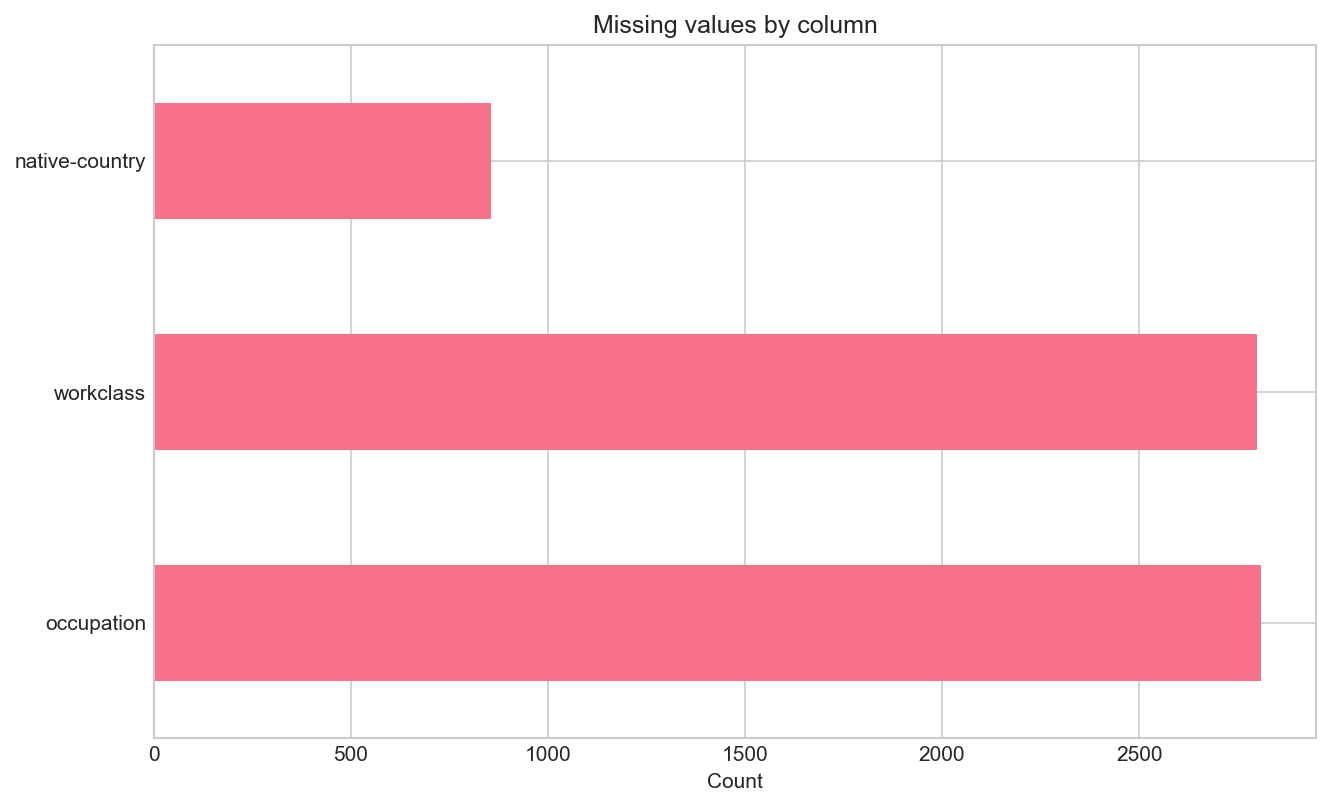
\includegraphics[width=0.9\linewidth]{figures/fig_01_missingness.png}
  \caption{Figure 1: Missing values by column}
\end{figure}

Figure 1. Missingness and unknown-category audit (EDA-001). Several categorical fields show missing values after replacing \texttt{?}.

\subsection{Task validity and limitations}

The Adult dataset reflects a specific U.S. census-era survey population. Labels are coarse (two income bands), and features may encode historical social structure. Results describe associative patterns in this dataset only; external validity to other populations or time periods is not claimed. See Section 19 and \texttt{reports/limitations.md}.


\section{Exploratory Data Analysis and Feature Selection}

\subsection{Feature roles}

Fourteen input features were retained: six numeric (age, fnlwgt, education-num, capital-gain, capital-loss, hours-per-week) and eight categorical (workclass, education, marital-status, occupation, relationship, race, sex, native-country). A full feature dictionary is in Table 2 (\texttt{table\_02\_feature\_dictionary.csv}).

\subsection{Missing values and distributions}

Figure 1 shows missing counts by column. Numeric features were summarised by income class (Figure 4). \textbf{Age}, \textbf{education-num}, and \textbf{hours-per-week} show visible separation between classes; \textbf{capital-gain} is sparse but informative for high earners.

\begin{figure}[H]
  \centering
  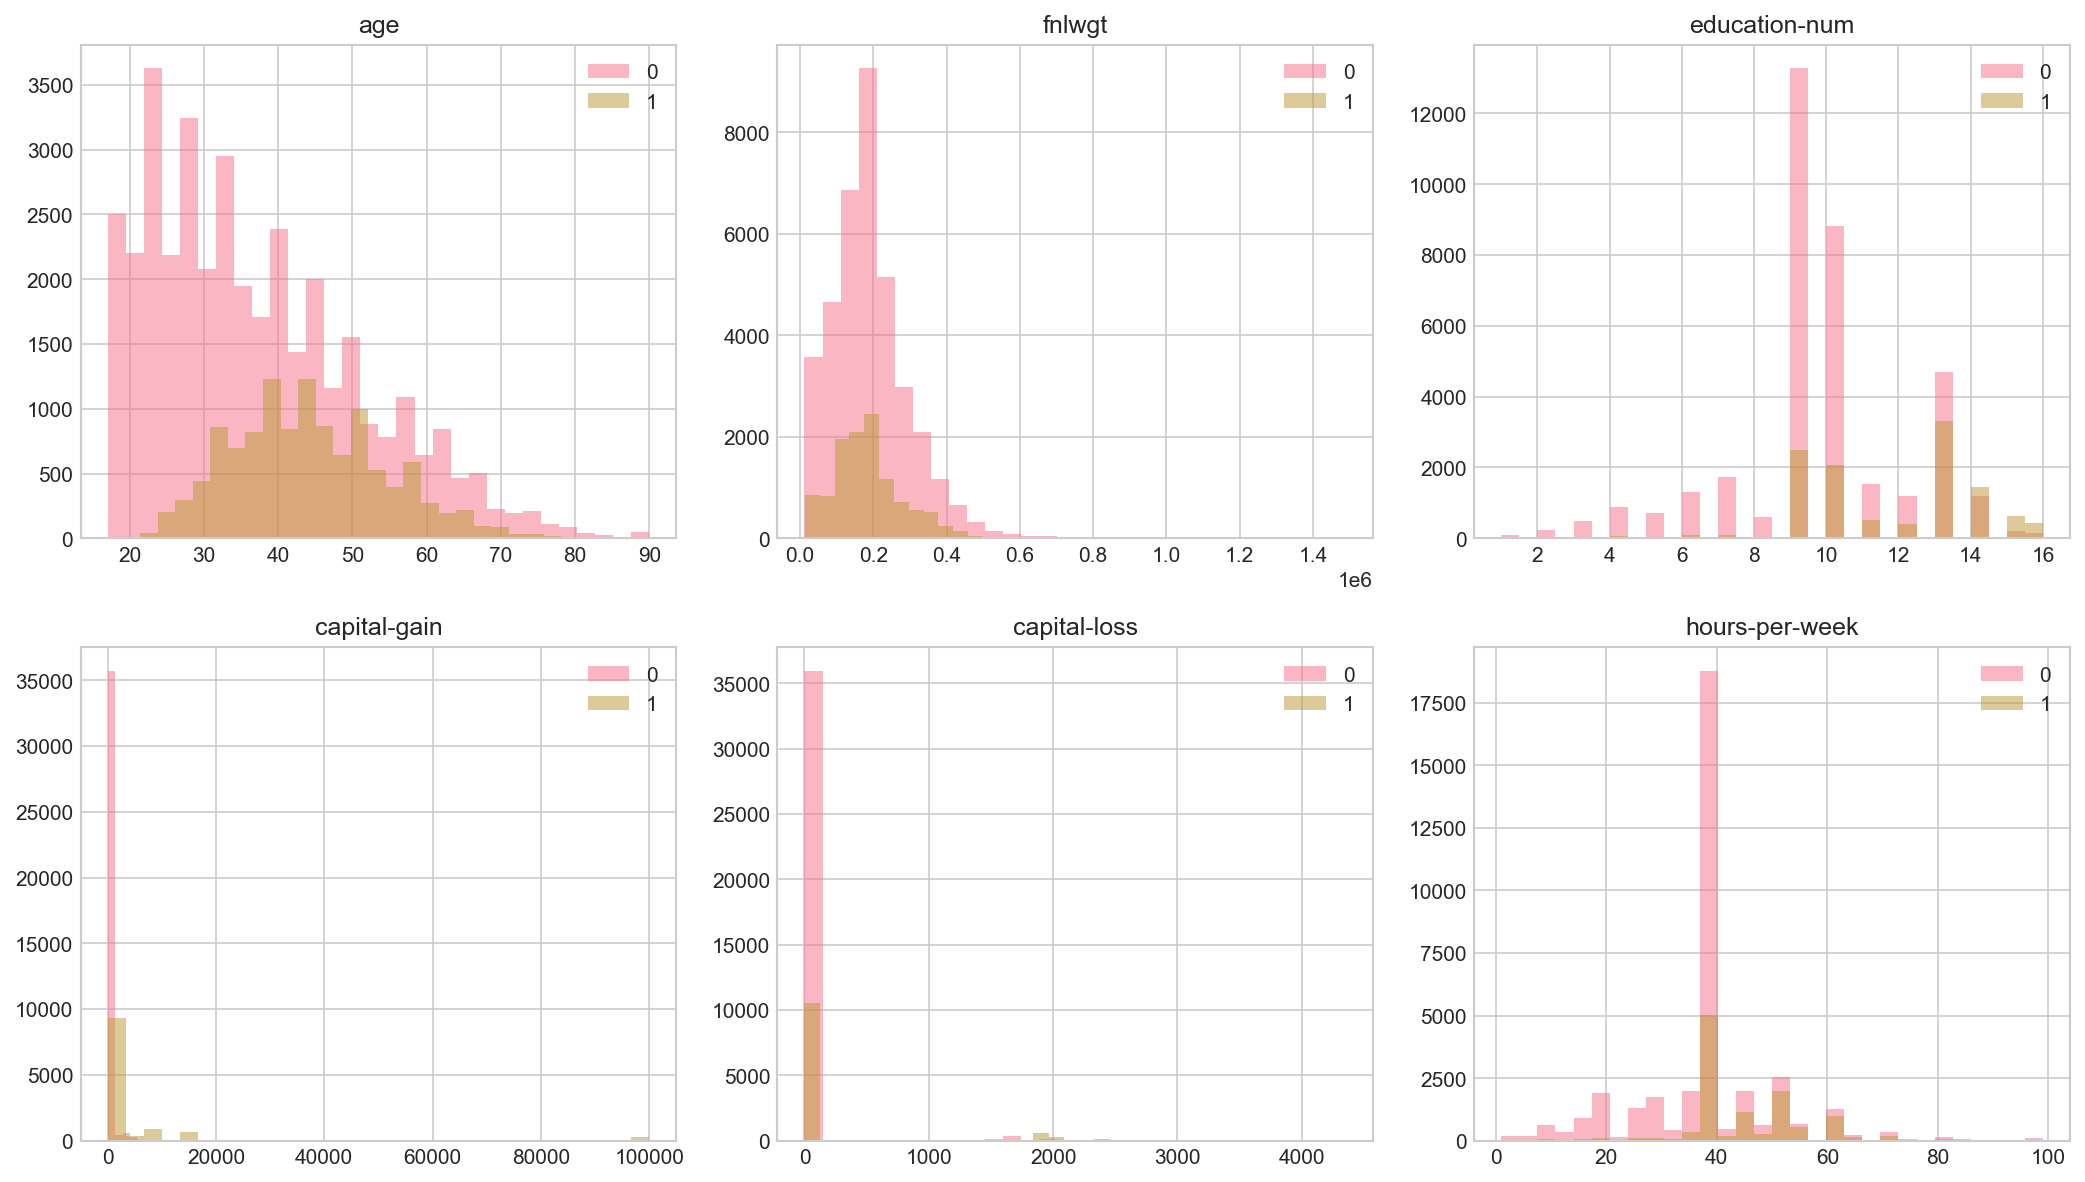
\includegraphics[width=0.9\linewidth]{figures/fig_04_numeric_by_target.png}
  \caption{Figure 4: Numeric distributions by target}
\end{figure}

Figure 4. Numeric feature distributions stratified by income label (EDA-001).

\subsection{Categorical associations and correlation}

High-income rates vary across education and occupation levels (Figure 5). Numeric features show moderate correlation (Figure 6); no feature was dropped solely for collinearity, as tree-based models handle redundancy and the pipeline preserves comparability across model families.

\begin{figure}[H]
  \centering
  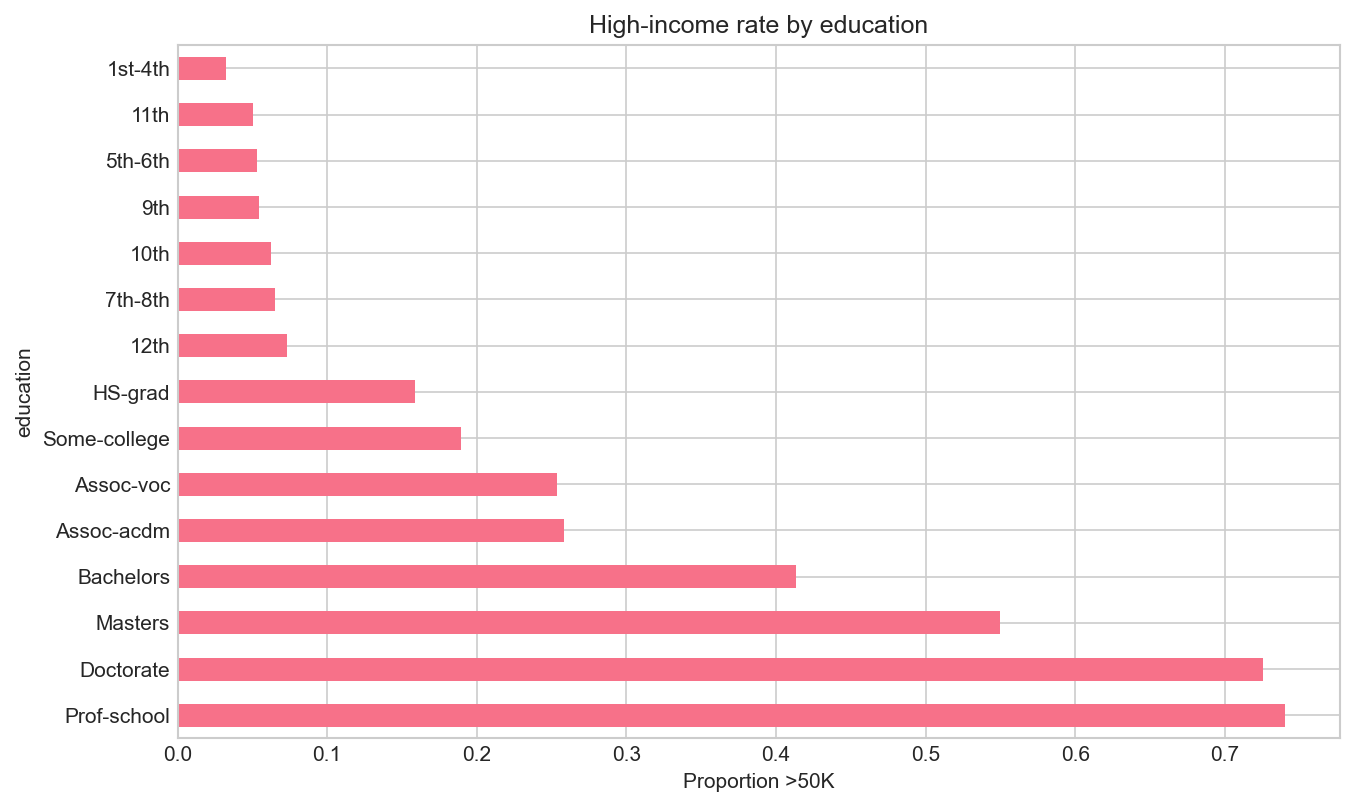
\includegraphics[width=0.9\linewidth]{figures/fig_05_categorical_rates.png}
  \caption{Figure 5: Income rate by education}
\end{figure}

\begin{figure}[H]
  \centering
  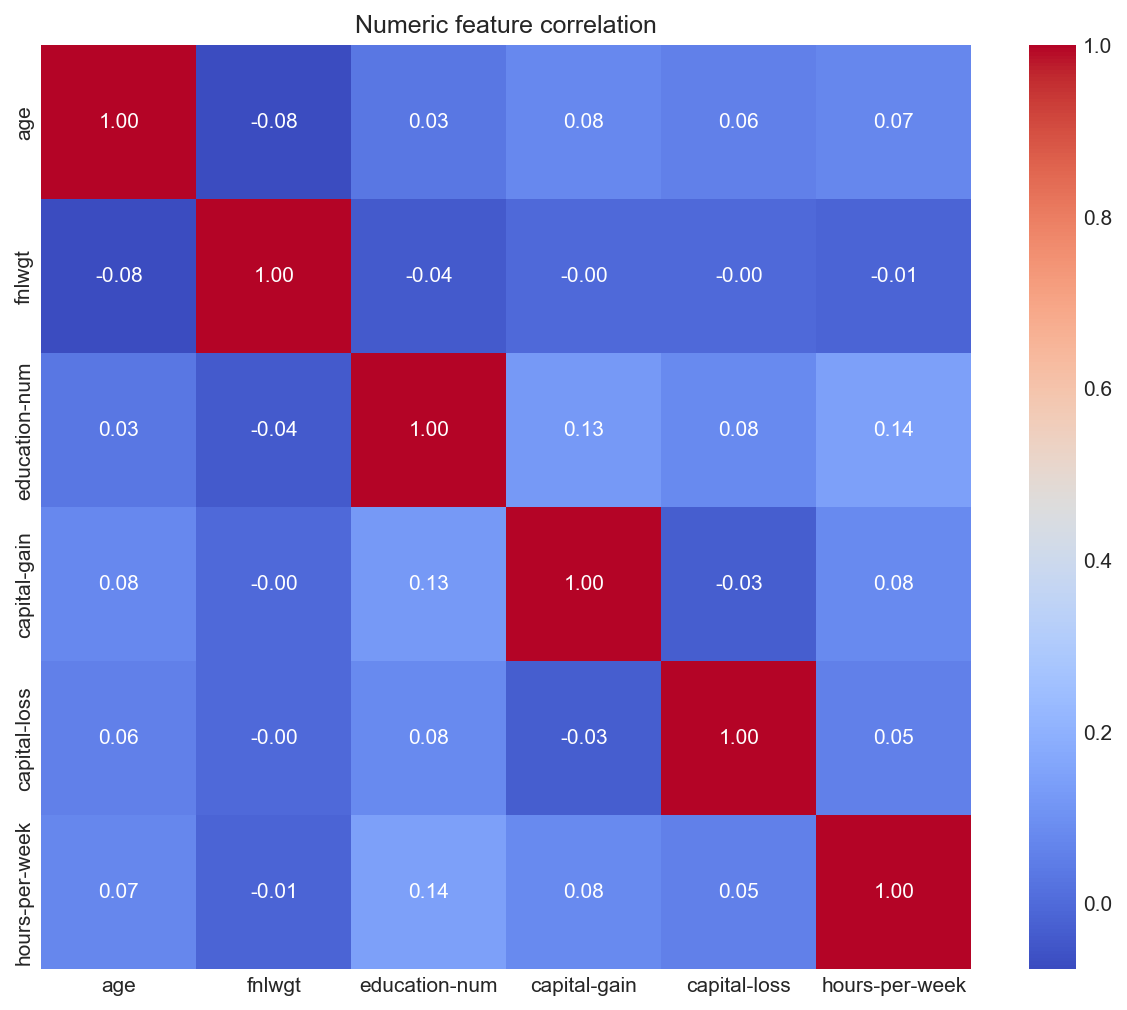
\includegraphics[width=0.9\linewidth]{figures/fig_06_correlation.png}
  \caption{Figure 6: Numeric correlation heatmap}
\end{figure}

\subsection{Feature selection decision}

No separate univariate filter was applied beyond EDA. All fourteen inputs feed a unified \texttt{ColumnTransformer} (median/mode imputation, standardisation for numeric fields, one-hot encoding for categoricals—FEAT-001). This keeps the modelling pipeline consistent and leakage-safe when nested in cross-validation.


\section{Target Balance and Sensitive Attribute Audit}

\subsection{Class imbalance}

Only \textbf{23.9\%} of records have positive class (income > \$50K). This imbalance motivates reporting \textbf{macro F1} and \textbf{balanced accuracy} alongside accuracy (EDA-002).

\begin{figure}[H]
  \centering
  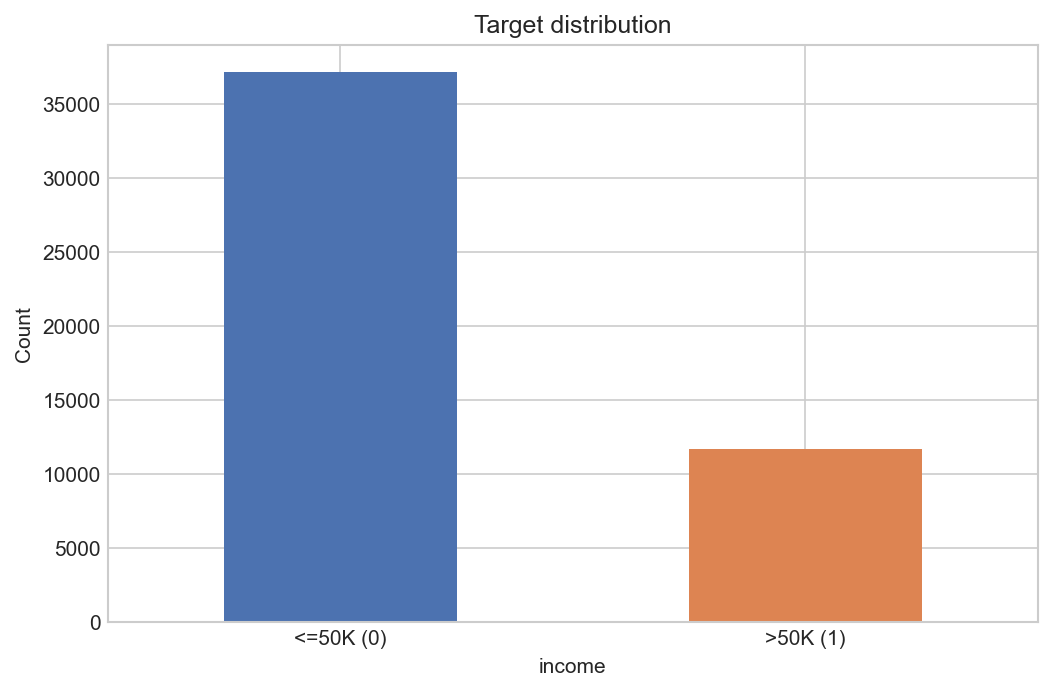
\includegraphics[width=0.9\linewidth]{figures/fig_02_target_distribution.png}
  \caption{Figure 2: Target distribution}
\end{figure}

Figure 2. Target class counts (EDA-002).

\subsection{Sensitive attributes}

\textbf{Sex} and \textbf{race} are designated sensitive attributes for fairness auditing (EDA-003). High-income rates differ across groups (Figures 3a–3b), indicating that models may learn group-correlated patterns. These attributes are \textbf{not} removed in the primary pipeline; Section 17 tests removal.

\begin{figure}[H]
  \centering
  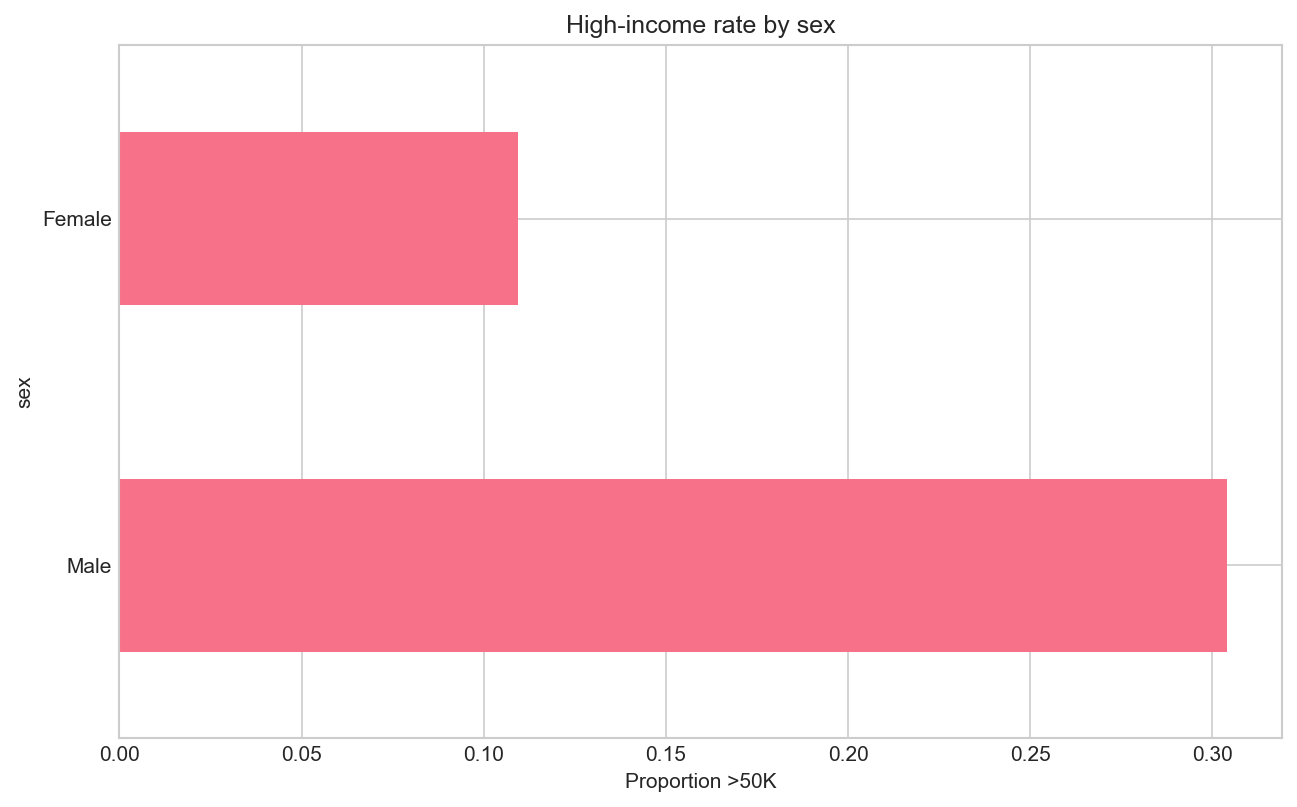
\includegraphics[width=0.9\linewidth]{figures/fig_03_sensitive_sex.png}
  \caption{Figure 3a: Income rate by sex}
\end{figure}

\begin{figure}[H]
  \centering
  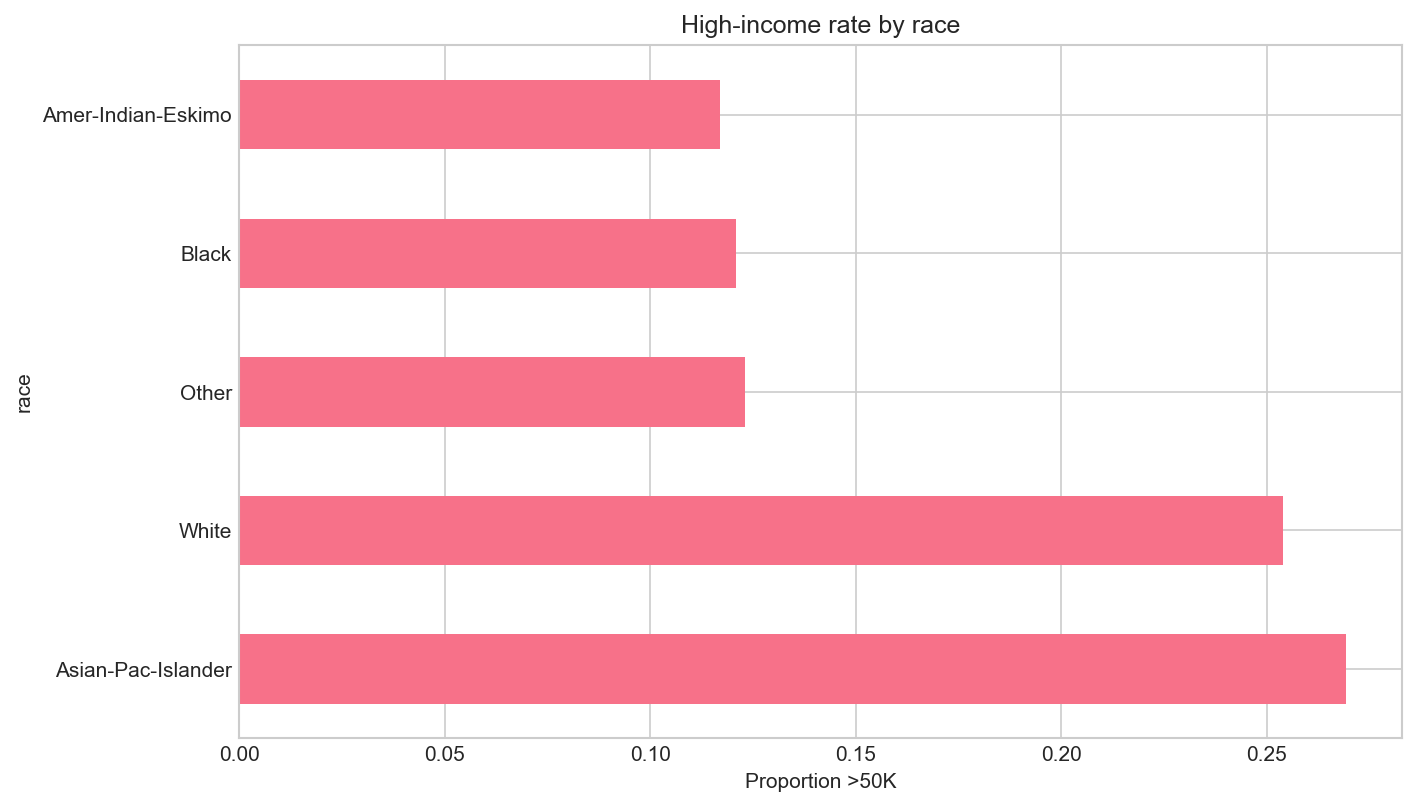
\includegraphics[width=0.9\linewidth]{figures/fig_03_sensitive_race.png}
  \caption{Figure 3b: Income rate by race}
\end{figure}

Figures 3a–3b. Proportion earning > \$50K by sex and race (EDA-003).

Imbalance and group rate differences foreshadow the need for macro-averaged metrics and subgroup diagnostics in later sections.

\end{document}
